\documentclass[11pt]{article}
\usepackage{fullpage,amsmath,mathtools, algorithm2e, forest}
\usepackage[mathletters]{ucs}
\usepackage{hyperref}
\usepackage[utf8x]{inputenc}
\usepackage{graphicx}
\usepackage{listings}
\usepackage{courier}

\lstset{basicstyle=\footnotesize\ttfamily,breaklines=true}
\lstset{frame=single}

\graphicspath{ {./images/} }
\title{COMP4107 - Assignment 3}
\author{Student Name: Yunkai Wang\\
\text{Student Number: 100968473}\\\\
Student Name: Jules Kuehn\\
\text{Student Number: 100661464}}
\date{Fall 2018}
\begin{document}
\maketitle
\begin{enumerate}

\item Question 1
\begin{enumerate}
\item
See q1.py for code. To see a comparison of input and output to the network, uncomment printVector() statements.\newline
\newline
In general, the fewer training images were used, the better the Hopfield network performed. These results suggests that a Hopfield network is a very poor choice for classification.\newline
\newline
A major factor in the accuracy was the selection of training images. Since fewer training images performed better, a random selection of a representative 1 or 5 leaves much to chance. To address this, we selected the training images with k-means, taking the images closest to the 2 cluster centers. This results in a selection of training images in which all 1's are very close to the center 1, and all 5's are very close to the center 5. Alternately, we tried taking as many cluster centers as training images, finding the closest image for each cluster center. This should result in selecting training images that maximally differ from each other.\newline
\newline
The graphs below compare classification accuracy against the number of images used to train the network, per digit. Each graph shows the average classification accuracy over 5 trials, with 50 test images.
\begin{figure}[h!]
    \centering
     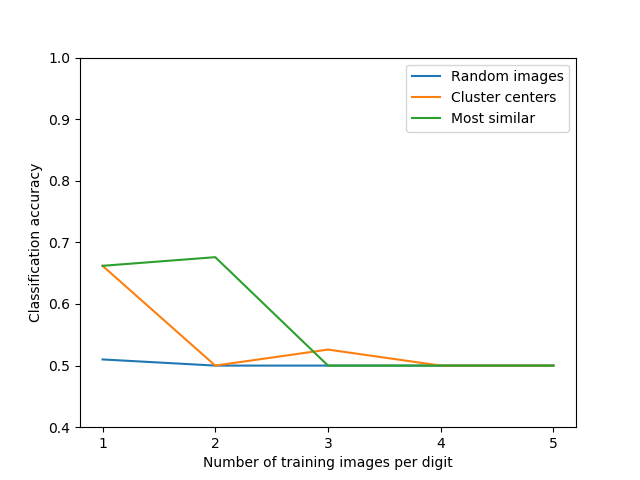
\includegraphics[width=0.5\textwidth]{q1_noStorkey}
        \caption{Hopfield classification of MNIST digits 1 and 5}
\end{figure}

\item
The code to implement the Storkey improvements are also included in our q1.py code. The Storkey algorithm slightly improves classification accuracy, but it is still unusable.
\begin{figure}[h!]
    \centering
     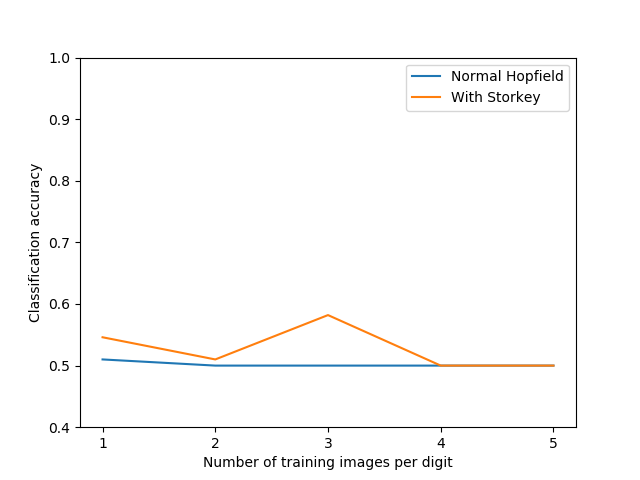
\includegraphics[width=0.5\textwidth]{q1_withStorkey}
        \caption{Hopfield classification with Storkey's rule}
\end{figure}
\end{enumerate}

\pagebreak

\item Question 2\newline
\newline
Our own implementation of K-means was used to generate centers and beta values for a Radial Basis Function neural network (implemented in q2.py). Training on a large proportion of the samples (63000 / 70000) yielded reasonable results (around 95\% classification accuracy) but was very slow. It was not practical use such a large training set for all the comparitive tests below, so the accuracy suffers.

First, the centers are initialized to a random training point. (Although the code allows for the initialization method suggested in class - creating a random point within the min/max of each dimension - this method wasn't as effective.) After running K-means, the centers and betas are used to compute RBF activations for the training and test data. This reduces the dimensionality of the input to the number of centers chosen. The RBF activations were then fed into a feed-forward neural net with no hidden layer, which was trained with the Adam optimizer. 3-fold cross-validation was used to produce the results below.
\begin{enumerate}
\item
Investigating a number of different sizes of hidden layer showed that the best value was around 160 centers. The graph below represents training for 100 epochs with no dropout, at a learning rate of 0.05, and with a sample size of 1000.
\begin{figure}[h!]
    \centering
     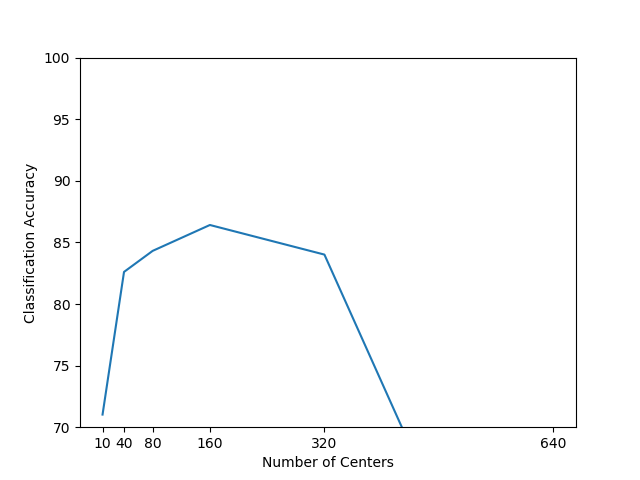
\includegraphics[width=0.5\textwidth]{q2_centers}
        \caption{Classification accuracy vs. hidden layer size}
\end{figure}

\item
Applying dropout before the output layer did not increase performance. We tested with the best case seen above (160 centers, 1000 samples, 100 epochs, lr=0.05) and also an "expanded" case (320 centers, 5000 samples, 500 epochs, lr=0.01). In both cases increasing the dropout level decreased the accuracy.
\begin{figure}[h!]
    \centering
    \begin{minipage}{0.45\textwidth}
    	\centering
        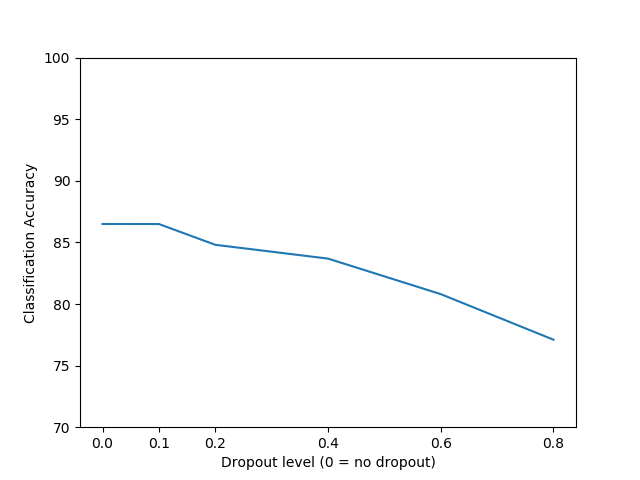
\includegraphics[width=0.9\textwidth]{q2_dropout1}
        \caption{Dropout with 160 centers}
    \end{minipage}\hfill
    \begin{minipage}{0.45\textwidth}
    	\centering
         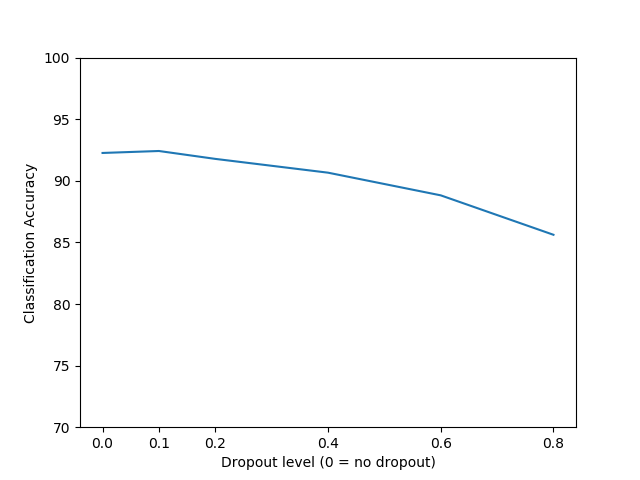
\includegraphics[width=0.9\textwidth]{q2_dropout2}
         \caption{Dropout with 320 centers}
    \end{minipage}\hfill
\end{figure}

\end{enumerate}

\pagebreak

\item Question 3

\begin{enumerate}
\item For part a, here are the parameters and dimension of the SOM computed. We used only 1024 samples to train the SOM, the reason for doing this is just to shorted the running time. Otherwise the SOM takes too long to converge. Since we are using 1024 samples, so we used a SOM of size $12 \times 12$. The $\sigma$ value is $1$, and the learning rate is $0.1$. Here is the graphs generated by using these parameters:\\
\begin{figure}[h!]
    \centering
    \begin{minipage}{0.45\textwidth}
    	\centering
        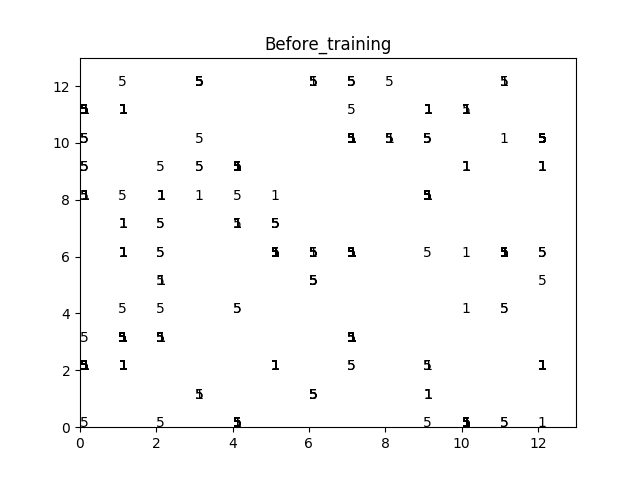
\includegraphics[width=0.9\textwidth]{Before_training}
    \end{minipage}\hfill
    \begin{minipage}{0.45\textwidth}
    	\centering
         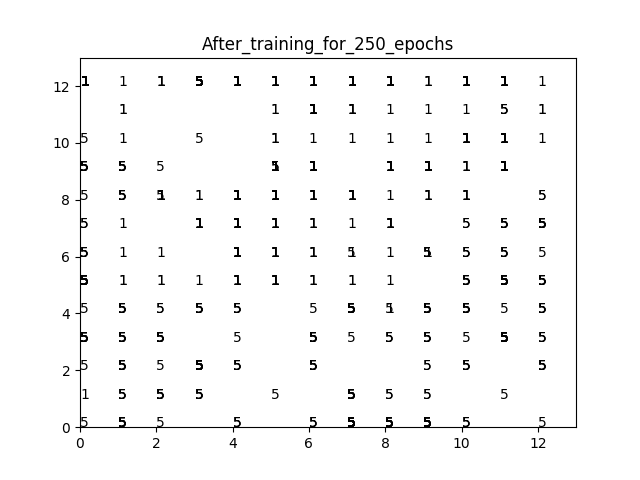
\includegraphics[width=0.9\textwidth]{After_training_for_250_epochs}
    \end{minipage}\hfill
    \begin{minipage}{0.45\textwidth}
    	\centering
         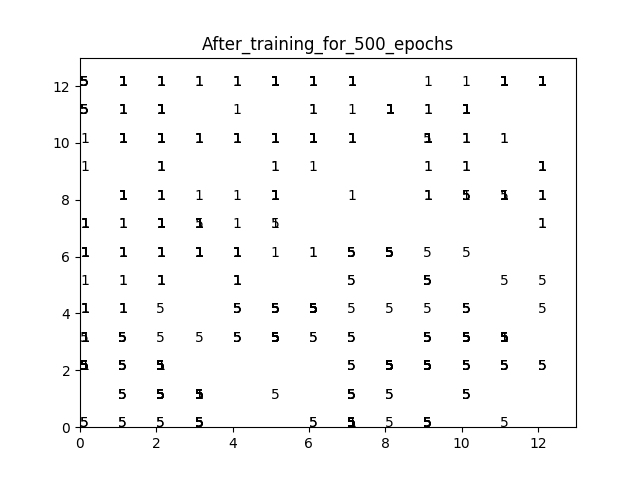
\includegraphics[width=0.9\textwidth]{After_training_for_500_epochs}
    \end{minipage}\hfill
\end{figure}
It's clear that as time proceed, the SOM starts to group all the 1's together, and all the 5's together, where initially the SOM was initialized randomly.

\item Here are the plots for the K-means solutions with different number of clusters.
\begin{figure}[h!]
    \centering
    \begin{minipage}{0.45\textwidth}
    	\centering
        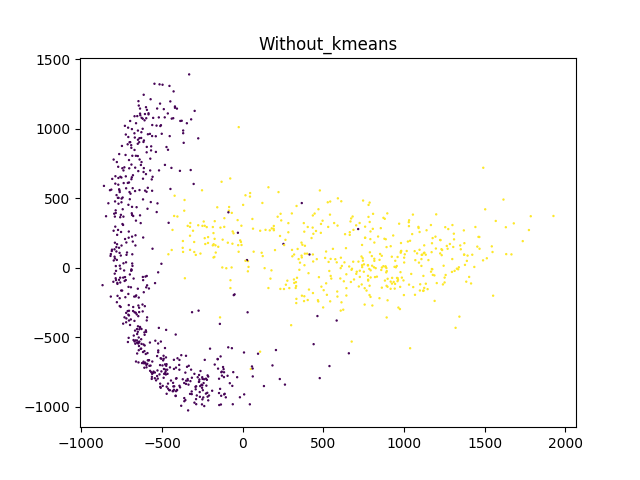
\includegraphics[width=0.9\textwidth]{Without_kmeans}
    \end{minipage}\hfill
    \begin{minipage}{0.45\textwidth}
    	\centering
         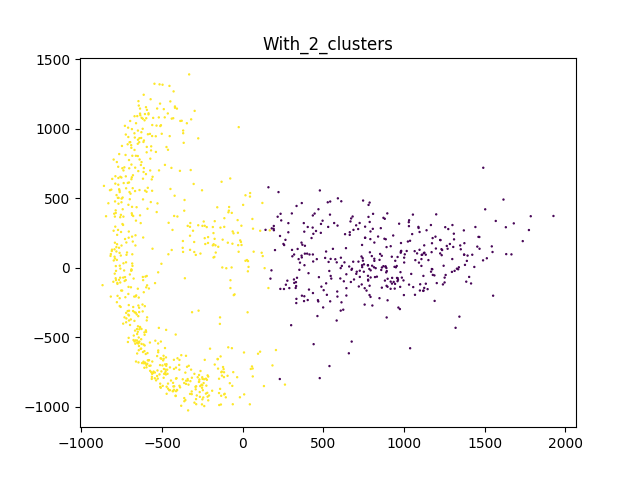
\includegraphics[width=0.9\textwidth]{With_2_clusters}
    \end{minipage}\hfill
    \begin{minipage}{0.45\textwidth}
    	\centering
         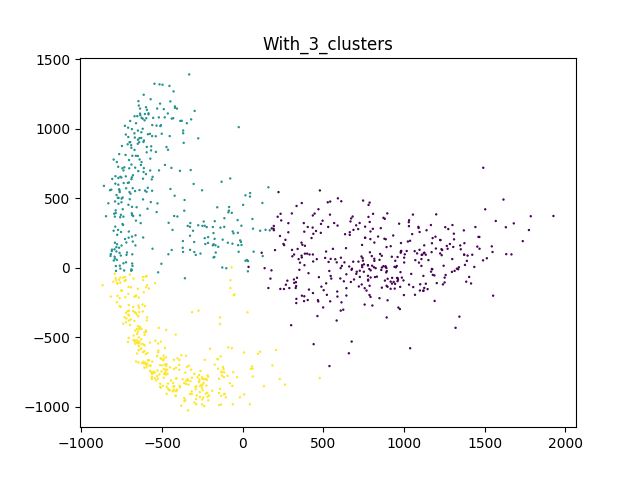
\includegraphics[width=0.9\textwidth]{With_3_clusters}
    \end{minipage}\hfill
    \begin{minipage}{0.45\textwidth}
    	\centering
         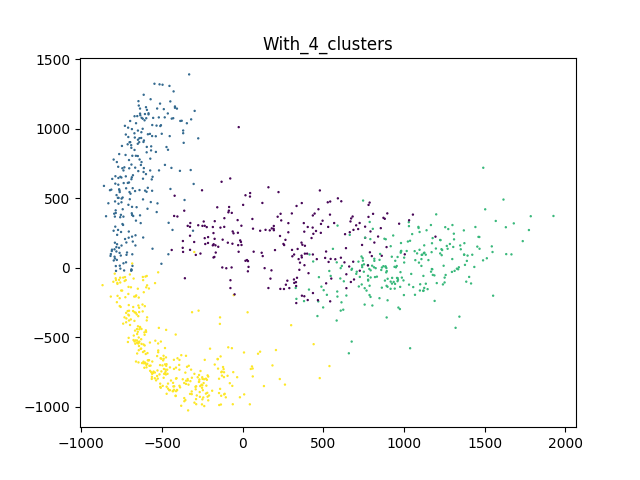
\includegraphics[width=0.9\textwidth]{With_4_clusters}
    \end{minipage}\hfill
    \begin{minipage}{0.45\textwidth}
    	\centering
         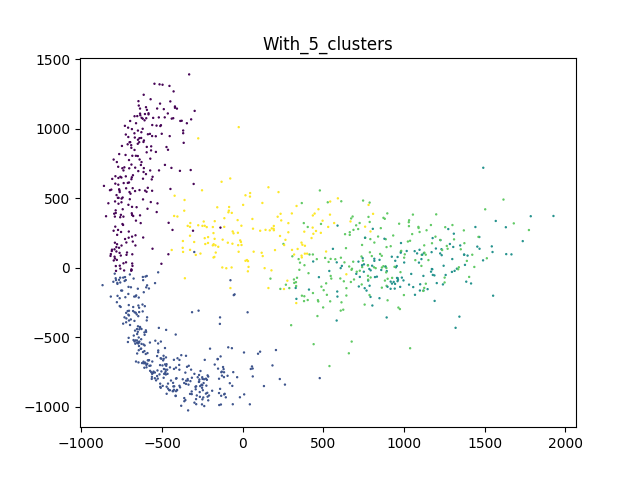
\includegraphics[width=0.9\textwidth]{With_5_clusters}
    \end{minipage}\hfill
\end{figure}

\end{enumerate}

\newpage
\item Question 4
\begin{enumerate}
\item We tried this question with two hidden layers, and we tried a different number of hidden layers for both layers. But the accuracy doesn't change for the different number of layers that we tried. The accuracy is always $9\%$ for all values that we tried. There may be some problem with the implementation we had.
\begin{figure}[h!]
    	\centering
        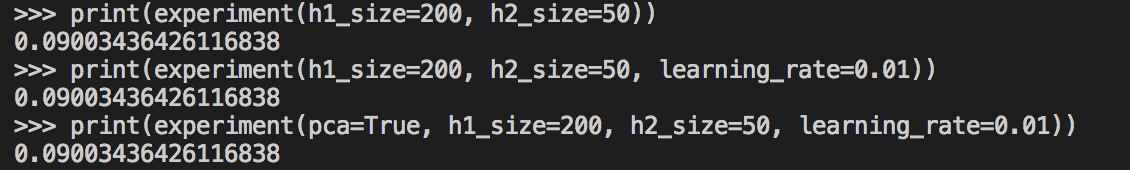
\includegraphics[width=0.9\textwidth]{q4}
\end{figure}


\end{enumerate}

\end{enumerate}
\end{document}